%%%%%%%%%%%%%%%%%%%%%%%%
%% Sample use of the infthesis class to prepare a thesis. This can be used as 
%% a template to produce your own thesis.
%%
%% The title, abstract and so on are taken from Martin Reddy's csthesis class
%% documentation.
%%
%% MEF, October 2002
%%%%%%%%%%%%%%%%%%%%%%%%

%%%%
%% Load the class. Put any options that you want here (see the documentation
%% for the list of options). The following are samples for each type of
%% thesis:
%%
%% Note: you can also specify any of the following options:
%%  logo: put a University of Edinburgh logo onto the title page
%%  frontabs: put the abstract onto the title page
%%  deptreport: produce a title page that fits into a Computer Science
%%      departmental cover [not sure if this actually works]
%%  singlespacing, fullspacing, doublespacing: choose line spacing
%%  oneside, twoside: specify a one-sided or two-sided thesis
%%  10pt, 11pt, 12pt: choose a font size
%%  centrechapter, leftchapter, rightchapter: alignment of chapter headings
%%  sansheadings, normalheadings: headings and captions in sans-serif
%%      (default) or in the same font as the rest of the thesis
%%  [no]listsintoc: put list of figures/tables in table of contents (default:
%%      not)
%%  romanprepages, plainprepages: number the preliminary pages with Roman
%%      numerals (default) or consecutively with the rest of the thesis
%%  parskip: don't indent paragraphs, put a blank line between instead
%%  abbrevs: define a list of useful abbreviations (see documentation)
%%  draft: produce a single-spaced, double-sided thesis with narrow margins
%%
%% For a PhD thesis -- you must also specify a research institute:
%\documentclass[phd,cisa,twoside,logo,parskip]{infthesis}

%% For an MPhil thesis -- also needs an institute
% \documentclass[mphil,ianc]{infthesis}

%% MSc by Research, which also needs an institute
% \documentclass[mscres,irr]{infthesis}

%% Taught MSc -- specify a particular degree instead. If none is specified,
%% "MSc in Informatics" is used.
% \documentclass[msc,cogsci]{infthesis}
 \documentclass[msc]{infthesis}  % for the MSc in Informatics

%% Undergraduate project -- specify the degree course and project type
%% separately
% \documentclass[bsc]{infthesis}
% \course{Artificial Intelligence and Psychology}
% \project{Fourth Year Project Report}

%% Put any \usepackage commands you want to use right here; the following is 
%% an example:
\usepackage{natbib}
%\usepackage{hyperref}
\usepackage{graphicx}
\usepackage{amssymb}
\usepackage{epstopdf}
\usepackage{parskip}
\usepackage{setspace} 
\usepackage{algorithm}
\usepackage{algpseudocode}
\usepackage{enumitem}
%% Information about the title, etc.
\title{Improving the discovery of Motifs in high-dimensional sequences of varying length}
\author{M. Adnan Haider}

%% If the year of submission is not the current year, uncomment this line and 
%% specify it here:
% \submityear{1785}

%% Optionally, specify the graduation month and year:
% \graduationdate{February 1786}

%% Specify the abstract here.
\abstract{%
    %This doctoral thesis will present the results of my work into the
    %reanimation of lifeless human tissues.
}

%% Now we start with the actual document.
\begin{document}

%% First, the preliminary pages
\begin{preliminary}

%% This creates the title page
\maketitle

%% Acknowledgements
\begin{acknowledgements}
Many thanks to my mummy for the numerous packed lunches; and of course to
Igor, my faithful lab assistant.
\end{acknowledgements}

%% Next we need to have the declaration.
\standarddeclaration

%% Finally, a dedication (this is optional -- uncomment the following line if
%% you want one).
% \dedication{To my mummy.}

%% Create the table of contents
\tableofcontents

%% If you want a list of figures or tables, uncomment the appropriate line(s)
% \listoffigures
% \listoftables

\end{preliminary}

%%%%%%%%
%% Include your chapter files here. See the sample chapter file for the basic
%% format.
\include{chapter1}
\chapter{Introduction}

Over the course of the last decade, the mining of time-series data have received considerable attention within the  data mining and machine learning community. The term 'time series' denotes a set of observations concurring any activity against different  periods of time. The duration of time period may be in the order of microseconds or monthly or even annually depending on the domain. Mathematically, a time series is defined by the values $y_1, y_2...y_n$ at times  $t_1,t_2... t_n$  where $y=f(t)$.  The time $t_i$  acts as an independent variable to estimate dependent variables $y_i$. The dimensionality of the  series is denoted as \textbf{n} where `\textbf{n}' denotes the length of the sequence. 

 Time series analysis is used in many applications ranging from  sales forecasting, budgetary analysis, stock market analysis and many more. One particular domain where the application of time series analysis is currently very popular is \emph{motif} discovery- the problem of efficiently locating frequent/interesting sub-patterns in the data.  The knowledge of motifs has been seen  to have important applications in various aspects of data mining tasks. For instance:

 \begin{itemize}
\item  The discovery of association rules  the reflect information of `primitive shapes[1].
\item  The clustering of data into meaningful subgroups.  Clustering is one of the most frequently used data mining tasks. It involves an unsupervised process  for partitioning  a dataset into meaningful groups. Such algorithms need to be specified on the initial seed of points and the number of cluster of groups. Motifs could potentially be used to address both 
problems. In addition, seeding the algorithm with motifs 
rather than random points could speed up convergence [17].
\item The identification of important sub-patterns in DNA and gene sequences[11]
\end{itemize}

In the analysis of speech data, motifs  also play a very important role. Recent research have shown that detecting and isolating motifs in speech  utterances is equivalent to extracting frequent spoken words or linguistic entities spoken by the speaker(s) [3,5]. These methodologies  are based on  understanding  the underlying structure of  the observed data and operate on the acoustic signal directly( i.e there is no intermediate recognition stage  to map the audio signal to a symbolic representation). This  allows  the word acquisition process to be unsupervised which is  completely a  different approach to the current speech recognition systems that are built using a supervised  training methodology employing  manually transcribed speech to model the underlying speech process.

   %Modern Speech recognition systems are typically built using a supervised training methodology that employs transcribed speech data to model the underlying speech process. Annotation of speech corpus are performed manually and are conducted at the level of phones. By a phone we refer to a unit of sound. Since annotation is performed at the level of phones, given the small duration of phones, it�s highly likely for annotators to miss phonetic boundaries or mislabel phone intervals. Hence the entire process of annotation is not only highly time-consuming but also prone to human error. Since the acquisition of labels is very expensive, the standard state of art systems are limited on their ability to be applied to new domains. To address this issue, recent research has been conducted  to develop systems that detect word entities through operating on the acoustic signal directly[3] i.e there is no intermediate recognition stage  to map the audio signal to a symbolic representation .   These methodologies rely of the location of motifs to identify frequently spoken word entities.

To identify and extract motifs from time series data, various clustering algorithms have been proposed. The most widely used and popular approaches include the use of:
\begin{enumerate}
\item Dynamic time warping  algorithm(DTW) [2,3,4,5,6,11] that clusters similar sequences separated by time shifts or temporal dynamics
\item Single value decomposition(SVD)12]. The entire time series data set can be approximated by a low-rank approximation matrix achieved through transforming the data into an orthogonal feature space  whose dimensionality is much lower than the original data sequences. 

\end{enumerate}
 But unfortunately, directly applying these clustering algorithms to the features i.e the individual time series points may not lead to appealing results. Although the DTW algorithm is immune towards patterns shifted in time or distorted in size/shape, the  time complexity of computing the DTW distance of two series is quadratic and is dependent on the dimensionality of the sequences or in other words the length of the sequences.  To address this issue, linear-time constrained versions of DTW (Itakura parallelogram[19], Sakoe-Chiba band[18]) are used to constraint the size of the search space but the use  of  such constraints impact the accuracy of the algorithm[20].

The SVD too, also suffers from similar problems. For data sets where the dimensionality of the data is much higher than the sample size, the computational cost associated with the factorisation of the matrix is quite large.  Apart from the computational cost, one of the main constraints of  applying SVD  is the requirement for  all samples to share the same dimension which  in the context of time series data means sequences must share the same length. This constraint greatly reduces the type of  time series domains to which SVD  can be applied to extract latent factors that denote motifs. The speech corpus is an example of one such domain. Data sets comprised of  speech utterances are a good example where recorded utterances do not share the same  dimensionality (i.e  the same length) and signals that are acoustically similar  may be a contracted/ expanded version of each other.  

%The Fourier transform  on the other hand, although like DTW can work with series of different lengths but is restricted by the fact that it is not time-localised[16]. For non-stationary  time series `signals' it is necessary to capture frequencies that are dominant at any given time.  Short-time discrete  fourier  transform tries to address this issue through some time-limited window centered on time  $t$. But using the window prevents good localisation of signal discontinuities.

The discovery of motifs in high dimensional time series data that vary in length  is still a difficult problem to work with. To address the drawbacks of DTW and SVD, there has been some recent work conducted to improve these algorithms. In the paper `` \emph {Fast time series classification using numerosity reduction}", the authors address the drawbacks of DTW in handling high dimensional sequences. They propose an adaptive approach that initially uses a strict window constraint to reduce the search space of DTW but then gradually increase size of the window by discarding samples from the training set. Although this methodology improves the time complexity of the dynamic time warping algorithm by heuristically discarding regions in the input space, it does not improve the algorithm itself. In the case of SVD, for high dimensional time series sequences which vary in length, the  data matrix  suffers in being  incomplete. Carelessly addressing only the relatively few known entries is highly prone to over �tting. Earlier works [21] relied on imputation to fill  in missing ratings and make the rating matrix dense. However, imputation can be very expensive as it significantly  increases the amount of data. In addition, the data may be considerably distorted due to inaccurate imputation. 

The goal of this project is to improve the performance of  these algorithms in handling time series sequences that  have dimensionality and vary in length . To be precise, in the first half of the project, I will be investigating data mining and machine learning methods to  improve the speed of the DTW algorithm without degrading the accuracy. And in the second half I will be ...

For this project, I will be using 3 time series data sets (details in chapter 2):
\begin{itemize}
\item TIGITS 
\item INLINESKATE
\item CINC\_ECG\_TORSO
\end{itemize}
For a majority portion of the analysis, the TIDIGITS corpus will serve as  the primary dataset used  to investigate the performances of different models. The reason being the TIGITS corpus consists of utterances of words spoken by different speakers. Since each  time sequence corresponds to a speech utterance spoken by a speaker, as result of environment, context and speaker differences the length of the time series sequences will not be the same. In comparison the sequences with each UCR data set share the same dimensionality i.e length. Furthermore, the length of the time series sequences on average is much higher in the TIDIGITS corpus than sequences of any data set in the UCR time series database.
 %The discovery of motifs in high dimensional time series data that vary in length  is still a difficult problem to work with. Current works have only tried to address the issue of high-dimensional spaces. The state of the art algorithms have been to designed to work on high-dimensional time series sequences that all share the same length. To my knowledge, there exits no algorithm apart from DTW that can applied to high-dimensional sequences varying in length.  Using this as motivation, the aim of this project is to investigate methods  that can improve the discovery of motifs in  high-dimensional time-series sequences that vary in length. In this project, I particularly focus on improving the performance of the DTW algorithm in high dimensional spaces and in the later chapters investigate on  how to adapt unsupervised parametric models to high dimensional  data sets  that vary in length. 

The  dissertation is  organised as follows: Chapter 2 gives a description of the 3 time-series datasets used for this project. Chapter 4  provides a detailed back ground description of the DTW algorithm. Chapter 3 and 4 investigates methods to improve the performance of the DTW algorithm in terms of both accuracy and speed. Chapter4...
\include{chap3}
\chapter{Datasets}
The primary dataset that I have used for this project is the `TIGITS' corpus. (I need to give more description here)

For Training : The entire training data is used
--To contain the computational complexitiy, I am usig samples from production 'a'


For the training set : 
To reduce the average mean time , I am using half of the training data set by choosing samples from one production:
I have chosen:

 225 samples from the boy category
 
 234 samples from the girl category
 
 495 samples from the men category
 
 513 samples from the women category
 

Note : the size of the training set is half of the original training set but contains examples of all classes [1-9]  

For the  test set : Due to the high computational complexity, I  am using only 1/3 of the test set
I have chosen 
162 random samples from boys

162 random samples from girls

326 random samples from men

326 random samples from women

Apart from the TIGITS, I have used two datasets from the UCR database:

The description of the data sets used for the next set of experiments are as follows:
  \begin{enumerate}
  \item CinC\_ECG\_torso
  
  \begin{itemize}
    \item Length of the time series:1639
  \item Size of test set:1380
  \item Size of training set:40
  \item Number of classes:4
  \end{itemize}
  \item  InLineSkate
  \begin{itemize}
    \item Length of the time series:1882
  \item Size of test set:550
  \item Size of training set:100
  \item Number of classes:7 
  \end{itemize}
 \end{enumerate}
  \include{chap2}

\chapter{DTW-Background}
The Dynamic Time Warping algorithm measures the similarity between  sequences varying in both time and speed. Formally, the problem formulation of the algorithm is stated as follows: Given two time series X, and Y, of lengths $|X|$ and $|Y|$,
\begin{eqnarray}
X &= &x_1,x_2...x_{|X|}\\
Y &= &y_1,y_2...y_{|Y|}
\end{eqnarray}
construct a warping path W
\[ W =  w_1, w_2...w_k \mbox{ where max } (|X|,|Y|\leq k\leq |X|=|Y|\]
\begin{itemize}
\item Here \emph{k} denotes the length of the warping path and the  mth element of the warping path is $w_l = (n_l,m_l) \in [1 : N]\times[1 : M] \mbox{for } l \in [1 : k]$ where $n_l$ is an index from the  time series X and $m_l$ is an index from the time series Y.
\end{itemize}
To  properly understand  the  mechanism of the DTW algorithm, the definition of some key terminologies  must first be stated:
 \begin {enumerate}
\item Warping path:
An (N,M)-warping path (or simply referred to as warping path if N and M are clear from the context) is a sequence $w= (w_1,...,w_k)$ with $w_l = (n_l,m_l) \in [1 : N]\times[1 : M] \mbox{for } l \in [1 : k]$ satisfying the following three conditions.
 \begin{enumerate}
 \item Boundary condition: $p_1 = (1,1)$ and $p_k = (N,M)$.
 The boundary condition enforces that the first elements of X and Y as well as the last elements of X and Y to be  aligned with each other. In other words, the alignment refers to the entire sequences X and Y.
 \item Monotonicity condition requires that  the path will not turn back on itself, both the i and j indexes either stay the same or increase, they never decrease. 
 
 \item Step-size condition: $p_{l+1}-p_l \in \{(1,0),(0,1),(1,1)\}$  for l $\in$ [1:k-1].
 The step size con- dition expresses a kind of continuity condition: no element in X and Y can be omitted and there are no replications in the alignment
 \end {enumerate}
 Intuitively speaking, the (N,M)warping path$ p = (p_1,...,p_k) $defines an alignment  between two sequences $X = (x_1,x_2,...,x_N)$ and $Y = (y)1,y_2,...,y_M)$ by assigning the element $x_i$ of X to the element $y_j$	of Y.   
 \item Optimum Warping Path :
 
 The optimal warp path corresponds to the  minimum-distance warp path, where the distance of a warp path W is given as 
 \[ Dist(W) = \sum_{i=1}^{K} dist(X,Y)_{|(w_i)}\]
 $dist(X,Y)_{|(w_i)}$  represents the distance computed using an appropriate  cost function between the time series points of $x_{ni}$ of sequence X and $y_{mi}$ of sequence Y. \[\emph dist(X,Y)_{|(w_i)} = dist(x_{ni},y_{mi}) \]
 
\end{enumerate}
The goal of the DTW algorithm is to compute the distance of the optimal warping path between two time series sequences. Instead of attempting to solve the entire problem all at once, the DTW algorithm utilises the technique of dynamic programming to find an optimum alignment between two sequences through the computation of local distances between the points in the temporal sequence. A two-dimensional $|X|$ by $|Y|$ cost matrix D, is constructed where the value at $D(i, j)$ is the minimum- distance warp path that can be constructed from the two time series $X=x)1,...,x_n $ and $Y=y_1,...,y_m$. 
\[D(i,j) =Dist(i,j) +min[D(i-1,j),D(i-1,j-1),D(i,j-1)\]

The figure below gives an example of the working the algorithm.
\begin{figure}[H]
  \centering
   
     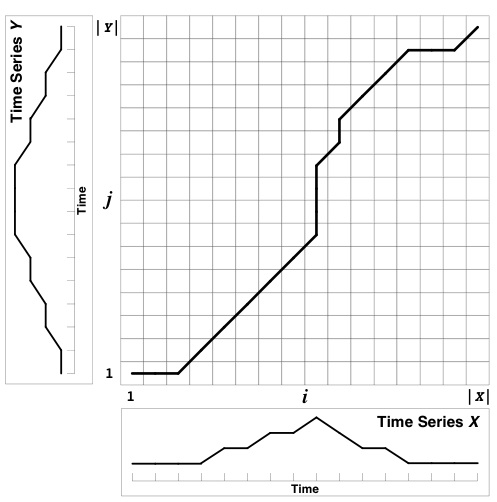
\includegraphics[scale=0.8]{DTWpicture.jpg}
  \caption{A cost matrix with the minimum-distance warp path traced through it.  }
  \end{figure}
\include{chap3}
\chapter{Improving DTW}
The Dynamic Time Warping(DTW) algorithm is the one of the oldest algorithms that is used to compare and cluster sequences varying in time, length and speed. Formally, given two temporal sequences, the algorithm utilises the technique of dynamic programming to find an optimum alignment between  through the computation of local distances between the points in each sequence. The time and computational complexity of this algorithm is  \emph{O}(mn) where $m$ and $n$ denote the length of the sequences that are being compared. Thus for  high dimensional time series sequences, the time and computational costs incurred by the algorithm are quite high which  makes DTW a very unattractive choice for clustering or discovering motifs in high dimensional  data sets.  Intuitively speaking, DTW is a clustering algorithm that clusters similar patterns varying in time and speed. Another drawback for working in high-dimensional spaces is the contrast between the distances of nearest and furthest points. The distances between such points  become increasingly smaller  as the dimensionality increases. This makes it  difficult to construct meaningful cluster groups in such spaces.

To address the issue of the curse of dimensionality, DTW algorithms employ a window constraint to reduce the search space. The window constraints determine the allowable  shapes that a warping path can take. As the dimensionality of the data increases, the size of the window is adjusted accordingly. Rigid  window constraints impose a more rigid alignment  that prevent an overly temporal skew between two sequences, by keeping frames of one sequence  from getting too far from the other. For clustering data sets such as speech utterances, the effect produced by such global constraints is highly undesirable. If we consider two utterances of a word spoken at different time frames, the patterns can have an overly temporal askew between them as result of the different contexts in which the  words are spoken and/or as a result of  different speakers speaking the same word. Thus it is necessary to explore techniques  other than window constraints that can improve the performance of the DTW algorithm in terms of both accuracy and time. 

 Before investigating methods to improve a technique, it is highly necessary to first understand the nature of the data itself. In this chapter, I investigate data-driven preprocessing techniques  that attempt to understand the underlying intrinsic structure of the lower-dimensional space on which the  data lives. By achieving a thorough understanding of the data,we can   achieve dimensionality reduction by  isolating and identifying smaller set of new(current)  features  that are more relevant for the problem in hand. 
 
 
 There are presently two groups of preprocessing techniques commonly used to address this issue:
\begin{itemize}
\item  Feature Selection 
\item Feature Extraction
\end{itemize}
 Feature selection techniques  involve selecting only a subset of attributes from the original data.  One of the most popular approaches to feature selection is  the exploratory data analysis(EDA). EDA is an approach to data analysis that postpones the usual assumptions about what kind of model the data follows with the more direct approach of allowing the data itself to reveal its underlying structure and models. The particular techniques employed in EDA are often quite simple, consisting of various techniques of:
 
 \begin{enumerate}
\item Plotting the raw data such as data traces, histograms, histograms, probability plots, lag plots, block plots, and Youden plots.
\item Plotting simple statistics such as mean plots, standard deviation plots, box plots, and main effects plots of the raw data.
\item Positioning such plots so as to maximize our natural pattern-recognition abilities, such as using multiple plots per page.
 \end{enumerate}
Feature extraction processes on the other hand are concerned with  a range of techniques  that apply an appropriate functional mapping to the original attributes to extract new features. The intuition behind feature extraction is that the data vectors $\{x_n\}$ typically lie close to a non- linear manifold whose intrinsic dimensionality is smaller than that of the input space as a result of strong correlations between the input features. Hence by using appropriate functional mapping, we obtain a smaller set of features that capture the intrinsic correlation between the input variable. Hence by doing so, we move from working in high dimensional spaces to working in low dimensional spaces. The choice  of appropriate functional mapping can  also improve the clustering of data as shown by figure 1:

In the rest of this chapter,  I explore a range of  feature selection and extraction methods  and investigate whether their application can improve the performance of the DTW algorithm in terms of both accuracy and time complexity.

\begin{figure}[h]
  \centering
   
     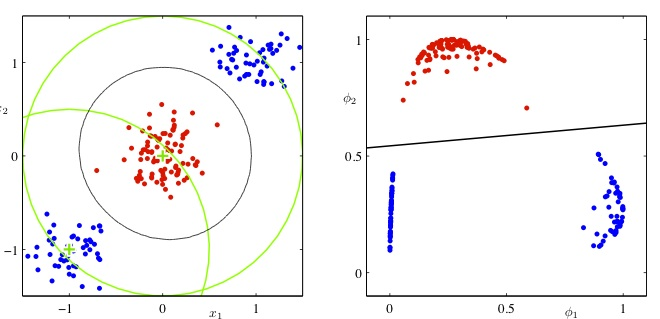
\includegraphics[scale=0.8]{featuremapping.jpg}
  \caption{The figure on the right corresponds to location of the data points in the feature space spanned by gaussian basis functions $\phi_1(x)$ and $\phi_2(x)$ }
  
\end{figure}

%The DTW algorithm combined  with the  1 nearest neighbour classifier  is a memory based algorithm. Memory-based methods involve storing the entire training set in order to make predictions for future data points. They typically require a metric to be defined that measures the similarity of any two vectors in input space, and are generally fast to �train� but slow at making predictions for test data points. The time and computational complexity associated with such methods is even higher when the dimensionality of the data points is high. Intuitively speaking, DTW is a clustering algorithm that clusters similar patterns varying in time and speed. In high- dimensional spaces, however, the contrast between the nearest and furthest points gets increasingly smaller, making it difficult to construct meaningful cluster groups. To address this issue, data dimensionality methods are used at the  preprocessing stage.
 
\section{Feature Selection}
The computational and time complexity associated with the DTW algorithm is governed by the dimensionality of the time  series. To get a feel of the data, I employed exploratory data analysis on the  isolated word utterances belonging to the test and training data sets  that I constructed from the TIDIGITS corpus. The aim here   to identify and isolate redundant features from the time series data.
 To get an idea about the structure of the data, I have studied the plots of the time series sequences along with performing auditory perception on the individual samples. Figure 2 gives the plot of raw signal corresponding to the word `8' by a speaker from the \emph{boy} category. From the visual and auditory analysis, I have made the following  observations:
\begin{itemize}
\item Long durations of silence occupy the beginning and end of each utterance.   These durations of silence segments are considerably long compared to the interesting regions in the acoustic signal that actually contain information about the spoken digit .  Removing these silence segments not only  reduce the dimensionality of the time series but also results in minimal loss of information.
\item  Through auditory perception of numerous samples, I have discovered that  the recordings are highly distorted when played in matlab even when the data is scaled so that the sound is played as loud as possible without clipping. The distorted signal fails to provide any time auditory clue about  category of the speaker i.e whether the speaker belongs to \{ boy,girl, men,women\}  and the signal must be played multiple times  for its class to be correctly identified.
\end{itemize}
\begin{figure}[h!]
  \centering
   
     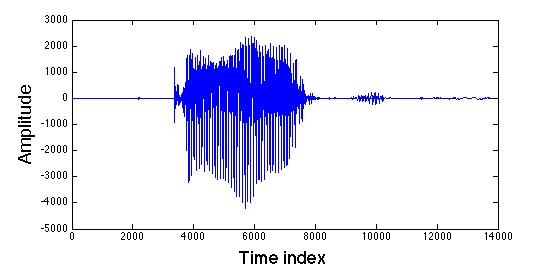
\includegraphics[scale=0.6]{Rawsample.jpg}
  \caption{`Raw 'signal}
  
\end{figure}
From  further experiments,  I have seen that if  I down-sample the utterances by $\frac{1}{2}$  which in other words means decreasing the sampling frequency by half, the resultant sampled signal is much clearer to understand. Sub-sampling  the utterances by half involves removing every other sample from the time series.  From the observation of figure 3, it can be sen that this technique  keeps the global trend of the signal intact but results in the  loss of local information. Furthermore through auditory perception of the sampled signals, I have discovered that losing some \textbf{local information} actually cleans the signal in a manner that allows the listener to identity the speaker's category and the utterance's class with ease.

With this knowledge  I have constructed  the following algorithm: `signal filter` that achieves  feature selection by removing segments of silence and downsampling the remaining segments by half.  An outline of the algorithm is as follows:

\begin{algorithm}[h]

\begin{algorithmic}[1]
\Procedure{SignalFilter}{$signal$}\Comment{raw signal }
\State $threshold=0$
\State maxAmplitude= max(rawSignal)
 \State Adapt the threshold based on the value taken by the maximum amplitude
 \State signalSil\_R$\leftarrow$ removeSilence(rawSignal,threshold)
 \State \textbf{return} output$\leftarrow$ downsample signalSil\_R by $\frac{1}{2}$
 
 \EndProcedure
\end{algorithmic}
 \caption{SignalFilter}
\end{algorithm} 
 \begin {itemize}
 \item The algorithm removes all samples in the times series sequence whose magnitude is less than the threshold. The threshold used is an adaptive parameter. By using the information of the signal's maximum amplitude the algorithm sets the threshold accordingly. It raises the threshold for signals corresponding to speakers having a loud and deep voice   and lowers the threshold for signals corresponding to speakers having gentle and low voice.
 \end{itemize}   
  
  
 \begin{figure}[H]
  \centering
   
     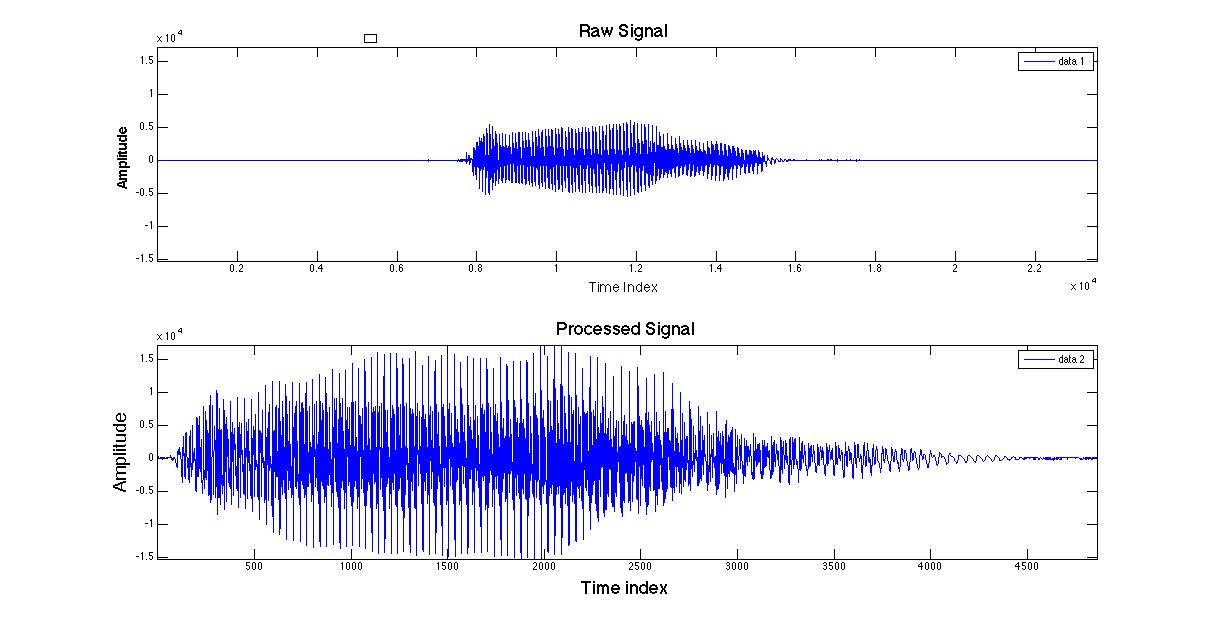
\includegraphics[scale=0.3]{Feature_selection.jpg}
  \caption{shows the raw acoustic signal corresponding to the utterances of the digit '5' alongside with the version that has its dimensionality reduced by the filter discussed above. From the comparison of the plots, it can be observed that the filter preserves the interesting patterns associated with the utterance while succeeding in reducing the dimensionality of the data.    }
  \end{figure}
  

 To analyse how introducing this feature selection process effects the performance of a DTW algorithm in working with high dimensional data, I have run the baseline value-added DTW(i.e DTW using raw values)  twice: once using the feature selection process as a preprocessing step and once without the feature selection process. An outline of the algorithm is given below.  
 \begin{algorithm}[H]

\begin{algorithmic}[1]
\Procedure{Value-based}{$seq1,seq2$}\Comment{two raw sequences }
 \State w = max($\lceil{0.1*max(n.m)}\rceil$, abs(n-m)) \Comment{Window constraint }
 \For{i=1: to length(seq1) }\Comment{Initialise the DTW cost matrix}
 \State DTW(i,0) = $\infty$
 \EndFor
 
 \For{i=1 to length(seq2)}
 \State DTW(0,i) = $\infty$
 \EndFor
 
  \For{i=2 to length(seq1)}  
 \For{j=max(2, i-w) to min(length(seq2), i+w)} \Comment { cost(a,b)$\equiv$euclid(a,b)}
 \State DTW(i,j) = cost(seq1(i),seq2(j)) + min\{ DTW(i-1,j)+DTW(i,j-1)+DTW(i-1,j-1)\}
 \EndFor
 
 \EndFor
\State \textbf{return}  result = $\frac{\mbox{DTW(n,m)}}{nm}$ \Comment{n=length(seq1), m=length(seq2)}

\EndProcedure 
\end{algorithmic}
\caption{Value-Based DTW}
\end{algorithm}
 
 The focus of my research here is to improve the accuracy of the DTW algorithm while reducing the time and computational cost to a minimum. Even after applying the feature selection process the dimensionality of the time series sequences is still very high. Thus for these experiments I have employed the most rigid window constraint   w = max($\lceil{0.1*max(n.m)}\rceil$, abs(n-m)) that keeps frames from one sequence  from getting too far from the other. The results found from the experiments are as follows:
 \begin{figure}[H]
  \centering
   
     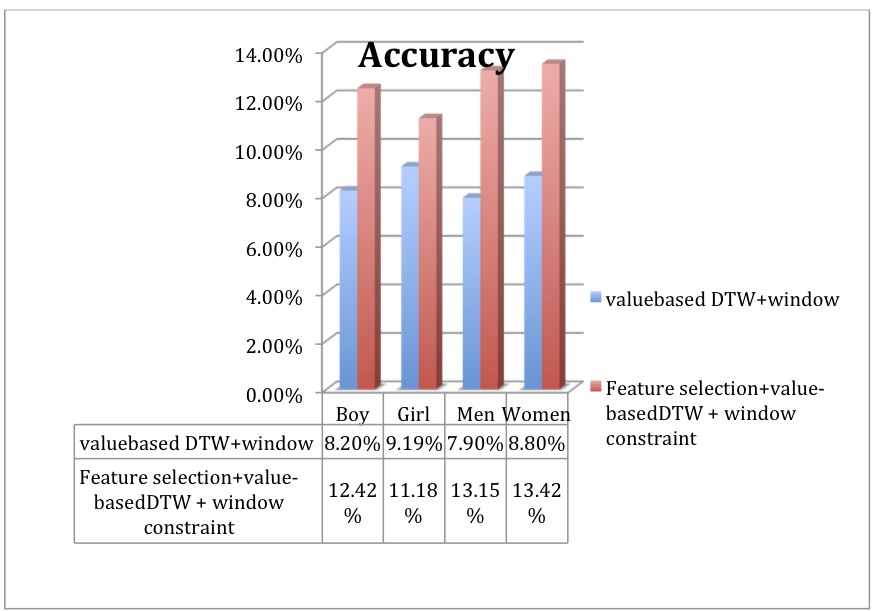
\includegraphics[scale=0.8]{value-basedaccuracy.jpg}
  \caption{ }
  
\end{figure}
\begin{figure}[H]
  \centering
   
     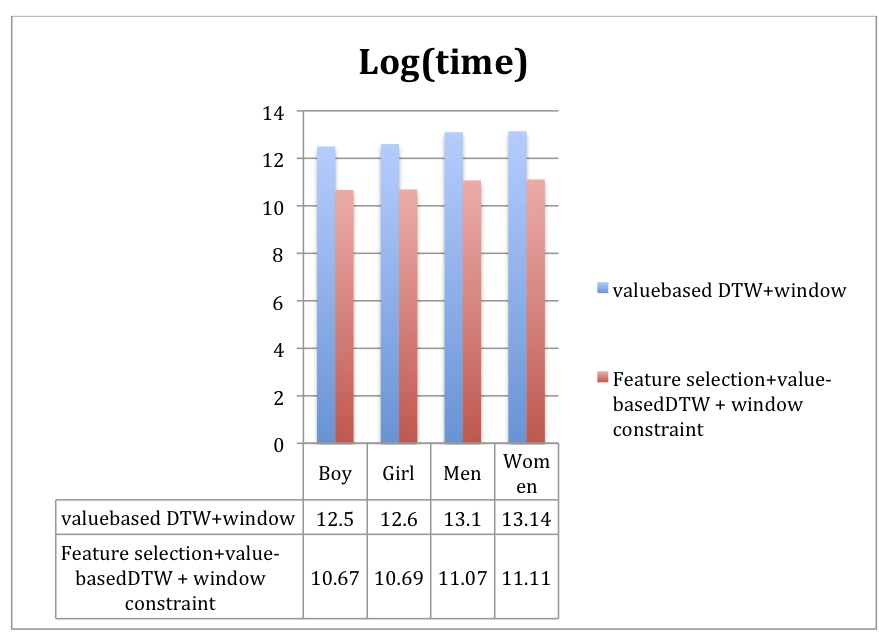
\includegraphics[scale=0.6]{value-basedtime.jpg}
  \caption{}
  
\end{figure}

Observations:
\begin{itemize}
\item Employing the prior feature selection process allows DTW subjected to global window constraint to improve both its accuracy and time complexity.

Explanations:
\begin{itemize}
 \item The DTW algorithm,due to  the high dimensionality of the  time series sequences is subjected to a window constraint that forces the algorithm to operate on the diagonal region of the DTW cost matrix. Removing  these redundant features increases the accuracy because these features  primarily represent segments of silence and since all utterances contain silence segments, taking these silences into account degrades the performance as  they bring i an unwanted notion of similarity in dissimilar patterns.
\item The size of the DTW cost matrix is \emph{O}(mn). Achieving dimensionality reduction through feature selection reduces the size of the cost matrix and thus decreases the computational cost.
\end{itemize}
\end{itemize}
\section{Feature extraction}
To improve the performance of the DTW algorithm even further, in this section I investigate domain-independent and domain dependent feature extraction methodologies  that employ an appropriate functional mapping to extract features that capture the intrinsic patterns of the data. The motivation behind this approach is to investigate to what degree we can improve the performance of the standard algorithm across different domains without making changes to the algorithm itself.

\subsection{ Domain-independent feature extraction}
The fundamental problem of baseline (value-based) DTW  is that the numerical value of a data point in a time series sequence is not a complete picture of the data point  in relation to the rest of the sequence. The context such as the position of the points in relation to their neighbours is ignored. To fix  this issue, an alternative  form of DTW know as \emph{Derivative} DTW is proposed but  it fails to achieve better performance across all domains as it ignores to take into account the common sub-patterns between two sequences(mainly global trends). Ideally we need to use features that contains information about the overall shapes of the sequences plus the local trend around the points. This allows the DTW to built a complete picture of the data point in relation to the rest of the sequence and hence achieve a better optimal alignment between the two sequences.

For feature extraction, the methodology that I have used  for this setup is based on Xie and Wiltgen's paper[]. In their paper, the authors highlight a domain-independent feature extraction process where each point in the time series sequence is replaced by a 4 dimensional vector. In this vector, the  first two features correspond to information regarding the local trends around a point and the last two features reflect the position of that point in the global shape of the sequence. From the experiments conducted on the UCR data sets, it has been observed that embedding DTW with this feature extraction process yields greater accuracy across all datasets. 

Definition of local feature given in [] is as follows:
\[ f_{\mbox{local}}(r_i)= (r_i-r_{i-1}, r_i-r_{i+1})\]



The  extraction of global features is constrained by two factors: the features that reflect information about  global trends and  the features must be in the same scaling order  as the local features. Being in the same scale allows them to  be combined with local features. In [] the authors used the following method to extract global features from the time series sequence:
\[ f_{\mbox{global}}(r_i)= (r_i -\sum_{k=1}^{i-1}\frac{r_k}{i-1} , r_i-\sum_{k=i+1}^M \frac{r_k}{M-i})\]

Note : The local and global features have no definition for the first and last points in a sequence.

When working with high dimensional time series data, the main drawback of employing this feature extraction method is that  it does not offer the advantage of  dimensionality reduction. The dimensionality of the feature space is just two dimensions less than the dimensionality of the original data. The DTW algorithm combined with this feature extraction process therefore suffers from the curse of dimensionality as before. To tackle this issue, as a prior step to the feature extraction process, I applied the  feature selection process that I have discussed in the previous section to remove  redundant features. 

The length of the resultant sequence of the vectors is still large. To address the issue of high computational cost, I have used the same window constraint applied the DTW algorithm equipped the two preprocessing stages of feature selection and extraction on the test data set that I had constructed from the TIGITS corpus. A summary of the results are given below:


\begin{figure}[H]
  \centering
   
     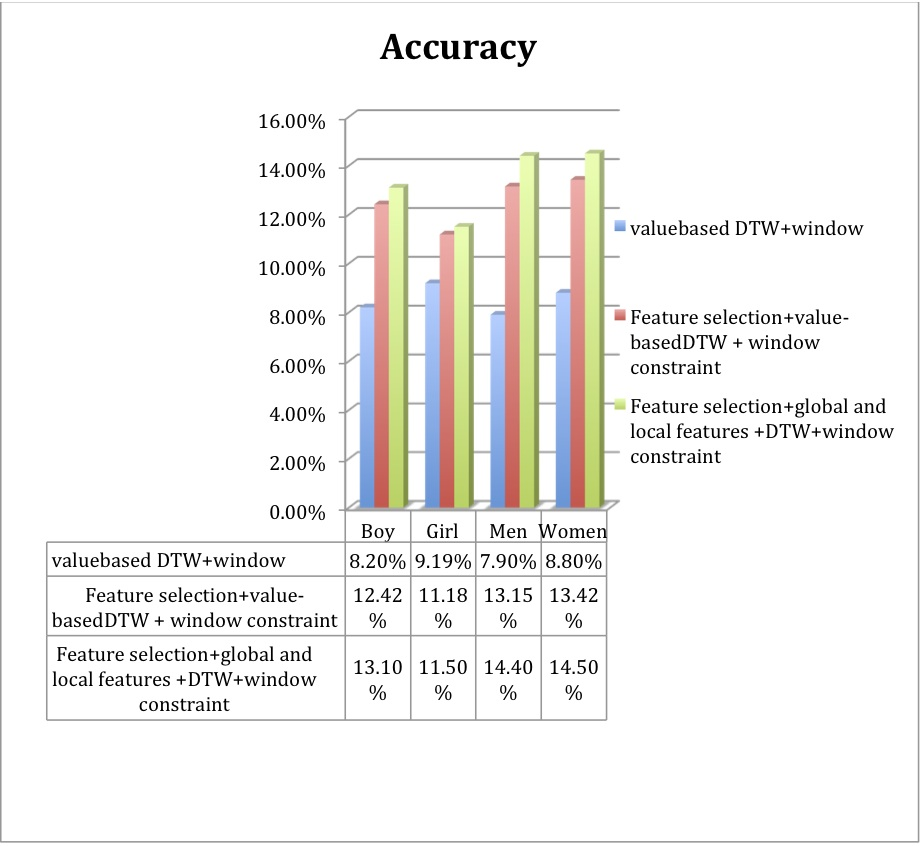
\includegraphics[scale=0.6]{localglobalaccuracy.jpg}
  \caption{}
  
\end{figure}
\begin{figure}[H]
  \centering
   
     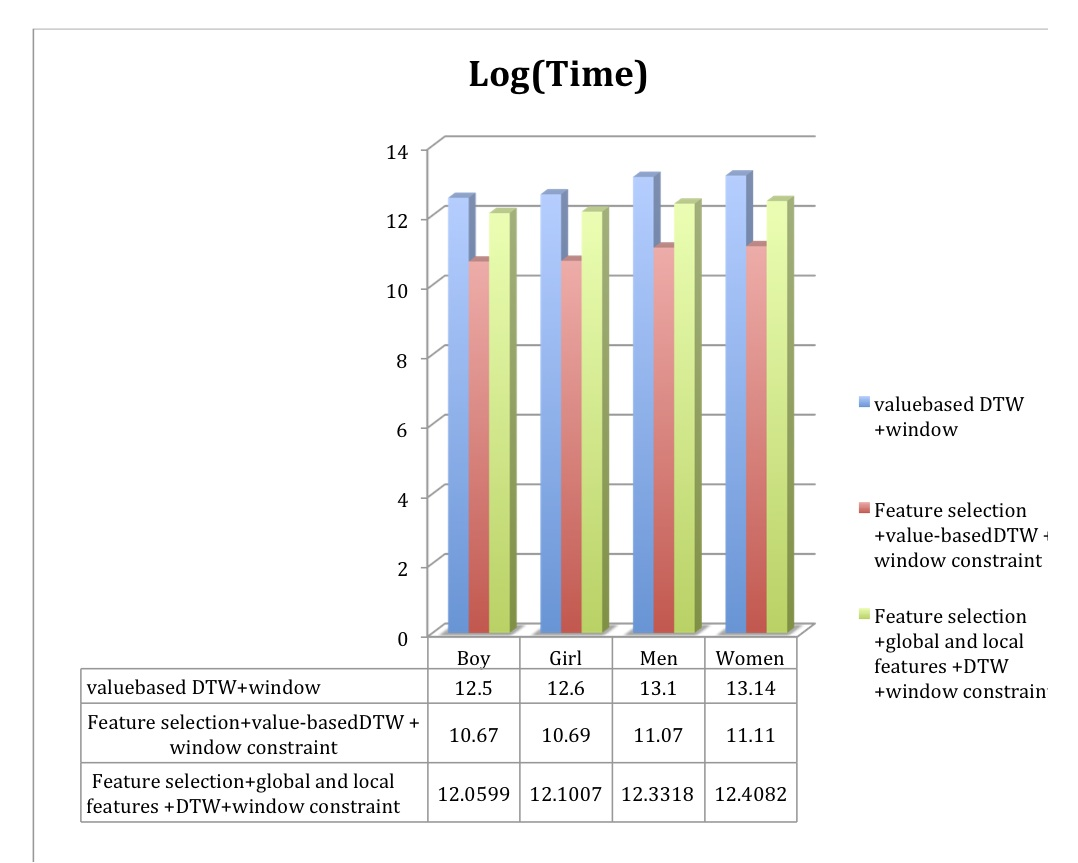
\includegraphics[scale=0.5]{localglobaltime.jpg}
  \caption{}
  
\end{figure}
Observation:
\begin{itemize}
\item Equipping DTW with a preprocessing stage that involves feature selection and extraction of local and global features result in a greater improvement in the accuracy of the algorithm.

Explanation:
\begin{itemize}
\item The algorithm now warps the time axis to  match the local and global trends  between points in the sequences instead of just their values. Since similar patterns will share the same trends, adding the feature extraction phase therefore improves the accuracy.
\end{itemize}
\item  The computational cost incurred by the algorithm is higher than the previous version that  uses  only the feature selection process.

Explanation:
\begin{itemize}
\item The cost of applying the euclidean metric on vectors $> $cost of applying the euclidean metric on points. Since the euclidean metric is applied $mn$ times. The overall computational cost increases.
\end{itemize}
\end{itemize}
The problem of working with a single data set is that if the model design is iterated many times using a limited size data set, then some over-fitting to the validation data can occur. To ensure that the models have not over-fitted to the test set, I ran the two versions of DTW :one that uses the preprocessing step of  feature extraction  while the other just uses the raw values for computing similarity, on the InlineSkate and Cinc\_Ecg\_Torso time series datasets[]. The results found are as follows:

Note: Both versions of DTW are equipped with the window constraint  w = max($\lceil{0.1*max(n.m)}\rceil$, abs(n-m)) to reduce the time and computational cost to a minimum.

\begin{figure}[H]
  \centering
   
     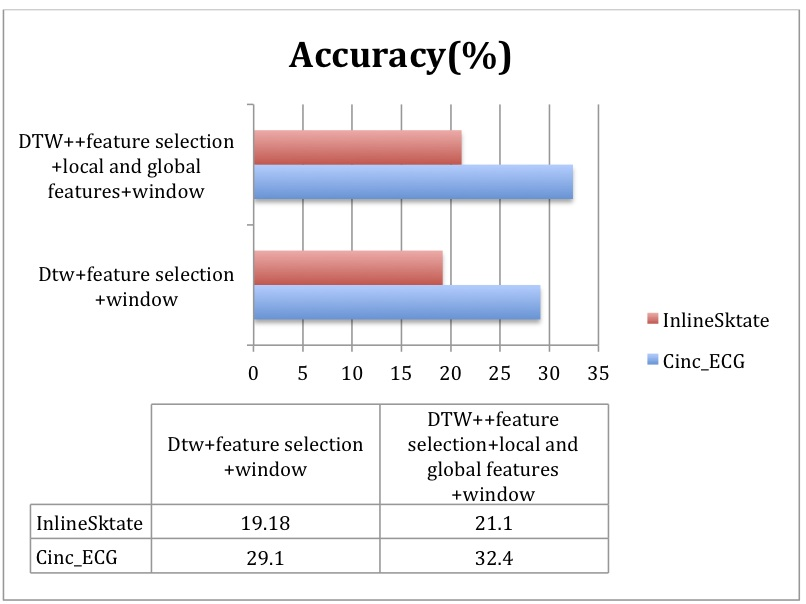
\includegraphics[scale=0.6]{cinc_inlineLocalGlobalaccuracy.jpg}
  \caption{}
  \end{figure}
\begin{figure}[H]
  \centering
   
     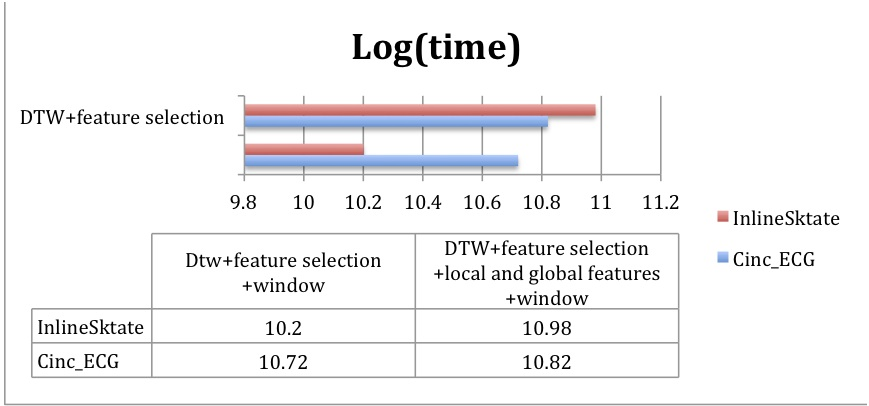
\includegraphics[scale=0.8]{cinc_inlineLocalGlobaltime.jpg}
  \caption{}
  \end{figure}
The differences between the two versions of DTW in terms of accuracy and time complexity are consistent  with the observations made in the previous experiment  with the TIDIGITS data set. This gives valid supports to the analysis of the tests that I  have conducted so far

\subsection{Domain-dependent feature extraction}

The main data set that I am working with is the TIGITS corpus which is composed of speech utterances. DTW formally is a domain independent algorithm.  It will  interesting to investigate to what degree is the  performance  of the algorithm effected if we model the information of the domain into the  DTW algorithm. Since at the moment, i am  investigating techniques that improve the performance of the DTW algorithm on high dimensional data without making changes to the algorithm itself, in this section, I investigate domain-dependent feature extraction methods that embed the  knowledge of the domain in  the feature extraction phase.  

For speech, the most commonly used features are the MFCC features-mel cepstrum ceptral coefficients.This feature representation is based on the idea of the cepstrum. For human speech, a speech waveform is created when a glottal source waveform of a particular frequency is passed through the vocal tract which because of its shape has a particular  filtering characteristic. The exact position of the vocal tract is in fact the key attribute in providing useful information about phones(units of sounds). Cepstrum provides a useful way to separate the information of the vocal tract from the glottal source.

A sketch of the MFCC feature extraction is given below:
\begin{figure}[H]
  \centering
   
     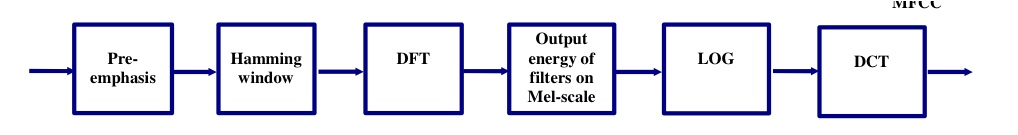
\includegraphics[scale=0.8]{mfcc.jpg}
  \caption{MFCC feature extraction}
  \end{figure}
\begin{enumerate}[label=\roman*]
\item Pre-emphasis: boosts the energy of the signal at high frequencies to improve phone detection
\item Windowing: partitions the time series sequence into frames using a hamming window
\item DFT: extracts spectral information at different frequency bands
\item Mel scale : transforming to mel scale improves recognition performance by allowing the model to take into account the property of human hearing
\item Log : makes the feature less sensitive to variations in input such as power variations on the speakers mouth.
\item Cepstrum : separate the information of the vocal tract from the glottal source. The first 12 cepstral values from spectrum of the log of the spectrum  are used
\end{enumerate}

Through the windowing process, the MFCC features extraction achieves dimensionality reduction. Each sequence is segmented into frames of length 20 to 30 ms which are then through appropriate functional mapping  are converted into sequences of MFCC feature vectors. Since the result sequence of vectors is much smaller than the length of the original sequence, the size of the DTW cost matrix is much smaller than before, This in turn lowers the time and computation cost incurred by the algorithm. One of the focal points of research for this project is to investigate alternative measures to using global window constraints that minimises the time and a computational  cost incurred by the DTW to  minimum without decreasing accuracy when working in high dimensional spaces. So  the question  that now lies is whether we can achieve greater reduction in dimensionality. The feature selection procedure that I discussed in the previous section reduces the size of the sequences by removing segments of silence followed the renaming segments by 1/2. As a prior step to MFCC feature extraction, if we use the first half of this feature selection process(i.e silence removal) and then  apply MFCC feature extraction, we achieve a dimensionality reduction which is greater than using either of the processes alone.

To test this idea I ran two versions of DTW on the TIGITS test set. The first version is equipped with a two step preprocessing stage: removal of silence followed by MFCC feature extraction while the 2nd version only employs MFCC feature extraction as pre-processing step. For this experiment, I had to impose a window constraint 
on the later version of DTW to contain the time and computational cost. Although MFCC feature extraction does achieve dimensional reduction. From doing initial tests, I have observed that the time taken by the algorithm to compare any two sequences is still  significantly high. To therefore reduce the computational time, I was forced to use the same window constraint that I employed for the previous experiments. A summary of the results of all experiments is given by the figures below:



\begin{figure}[H]
  \centering
   
     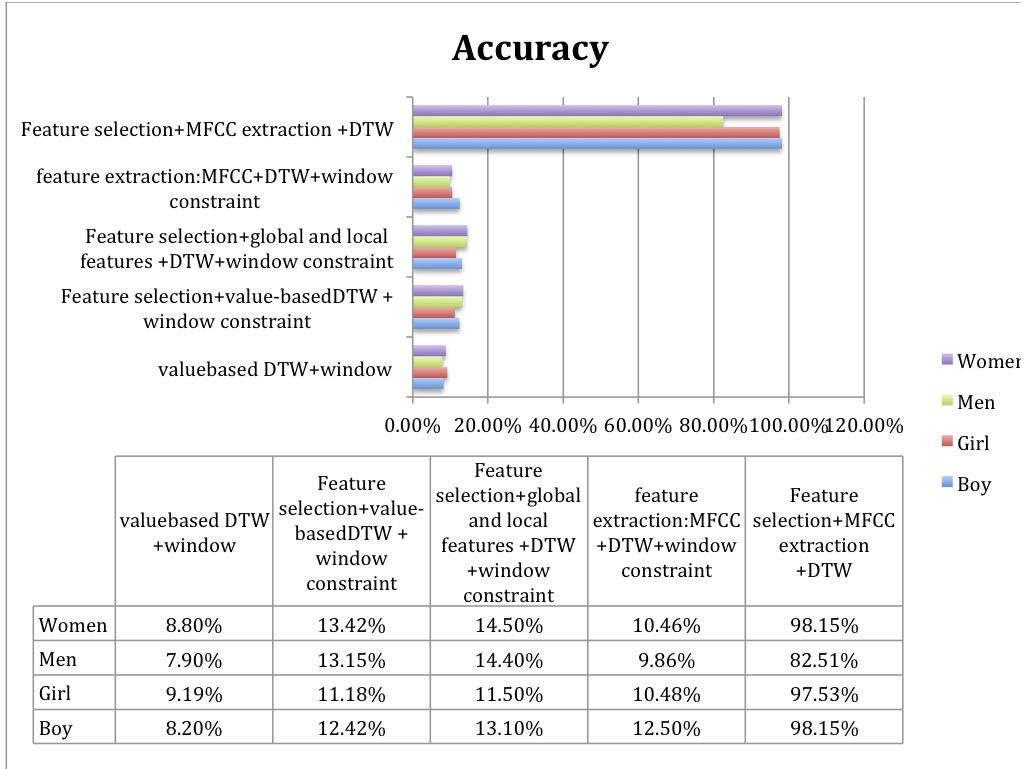
\includegraphics[scale=0.8]{Mfcc-accuracy.jpg}
  \caption{MFCC feature extraction}
  \end{figure}
  
\begin{figure}[H]
  \centering
   
     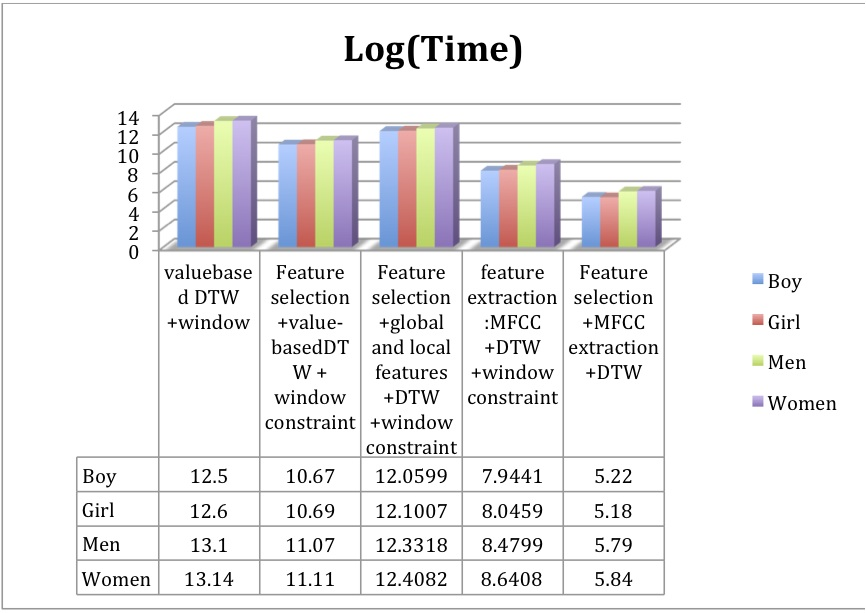
\includegraphics[scale=0.6]{Mfcc-time.jpg}
  \caption{MFCC feature extraction}
  \end{figure}
  Observations:
  \begin{itemize}
  \item It can be observed that adapting DTW to incorporate a pre-processing stage that involves removal of redundant features through silence removal and employing a feature extraction mapping that integrates domains knowledge in the feature extraction process achieves almost perfects accuracy and incurs the lowest computational time. To be precise, adapting DTW to be domain-dependent allows the algorithm to achieve near perfect accuracy while incurring the minimum computational cost. 
  \item From analysing the time complexity associated with each of the two versions, it can be seen that partitioning the sequences into frames actually leads to greater reduction in dimensionality of the time series than removing redundant features.
  \end{itemize}
  
To summarise, from the observation of the  results gathered from the  experiments it can be concluded that employing preprocessing steps that include the domain knowledge greatly improves the accuracy and time complexity of the DTW algorithm when high dimensional spaces and in some domain such the TIGITS corpus eliminates the necessity of impose global window constraints to achieve minimum computational cost.

 \include{chap4}
 \chapter{Adaptive DTW}
 n the previous chapter, I have investigated techniques on different pre-processing strategies that can improve the performance of the general  DTW algorithm  in working with high dimensional time series datasets. These techniques that I am investigated so far primarily focus on the improving the quality of the data rather than the algorithm itself. The results found from the experiments so far, have shown that understanding the intrinsic properties of the data and factoring in the  domain information can not only improve the performance of the  DTW but may even discard the need for a  the  global windowing constraint(as we have seen for the model that augments feature selection and MFCC feature extraction) to reduce the time and computational complexity.  The DTW algorithm is a memory based algorithm that employs a similarity metric to compare a sequence with all sequences in the training in an iterative manner.  Since the whole training set is used during the testing phase, the computational complexity makes the algorithm very attractive to use. The computational cost of a DTW algorithm is $(mn)$ where $m$ and $n$ denote the length of the two time series sequences currently being compared. Using longer sequences increases the size of the DTW cost matrix hence resulting into a greater number of computations. The domain-dependent pre-processing methodology doesnt guarantee the dropping of the  global window constraint that is used to reduce the search space when tackling high dimensional data. As we have seen from the experiments,when working with high-dimensional time-series data, the accuracy of the DTW algorithm using a window constraint suffers greatly even if it's equipped with domain dependent/independent features. Hence from a scientific point of view, it is of great interest to research methods to improve the DTW algorithm so it can constraint the time and computational complexity associated with high-dimensional data without degrading the accuracy by too much. In this chapter, I investigate an unsupervised methodology that:


 %Time series sequences are embedded with local and global trends. Unsupervised methods using DTW  focus on  exploiting the information of either these trends for pattern extraction and mining. From the  work conducted by Xie and Wiltgen on  the time series datasets[], it  has been shown that using DTW equipped with features that incorporate  information of \textbf{both}  local trends and global shapes in the clustering /classification process greatly improve the performance of DTW . Unlike the MFCC, the features constructed from local and global trends are domain independent and thus can be applied to any time of data.  However, when working high-dimensional time-series data, the accuracy of the DTW algorithm using a window constraint suffers greatly even if it's equipped with domain dependent/independent features. Hence from a scientific point of view, it is of great interest to research methods to improve the DTW algorithm so it can constraint the time and computational complexity associated with high-dimensional data without degrading the accuracy by too much. In this chapter, I investigate an unsupervised methodology that:

\begin{itemize}
\item incorporates  information about local and global trends  in the feature extraction process
\item employs an adaptive DTW that tackles the issue of the large time and computational complexity by moving from working on  time series sequences to  sequences of segmented time-slices. To counter the tradeoff in the decrease  in accuracy, the algorithm is equipped with a kernel function(self-proposed) that is designed to measure the similarity of sub-sequences more accurately than standard euclidean metric by being invariant toward time-dilation and scale.   
\end{itemize}

\section {{Feature extraction}}


For feature extraction, the methodology that I have used  for this setup is based on Xie and Wiltgen's paper[] that I have already discussed in the previous section.  Each point in the time series sequence is replaced by a 4 dimensional vector  where the first two features correspond to information regarding the local trends around a point and the last two features reflect the position of that point in the global shape of the sequence.
Definition of local feature as  given in [3.2.1] :
\[ f_{\mbox{local}}(r_i)= (r_i-r_{i-1}, r_i-r_{i+1})\]

Definition of global feature:
\[ f_{\mbox{global}}(r_i)= (r_i -\sum_{k=1}^{i-1}\frac{r_k}{i-1} , r_i-\sum_{k=i+1}^M \frac{r_k}{M-i})\]
\section{Adaption of DTW}
The feature extraction methodology discussed above maps the time series sequence to a time series sequence of vectors whose length  is $\|X_n\|-2. $   ( where $\|X_n\| $ denotes the  length of the original time series sequence).  The DTW augmented with these features will still suffer from large time and computational complexity if the dimensionality of the data is high. In the MFCC feature extraction process, the time series sequence is first segmented into series of frames  of length 20ms. Through appropriate functional mapping, each  frame is then mapped to a vector. Because the length of the resultant sequence of vectors is much smaller than the length of the original time series, the size of the  DTW cost matrix is reduced resulting in lower  time and computational cost associated with each comparison.

Similar to the MFCC extraction process, the time series of 4d vectors extracted in the feature extraction stage are segmented using windows  of width 5ms. The original time series is reduced to series of matrices  where the length of the new  series is 5 times smaller than before. Now if we adapt the cost function of DTW to work on series of matrices rather than series of vectors we can achieve a large improvement in the time and computational cost  associated in the testing phase without imposing a \textbf{window} constraint. 

The problem now can be shifted to finding  an appropriate kernel that can be used to compute the similarity between matrices composed of feature vectors. Ideally, we want a metric that takes into account the variation of speed and time when comparing two similar subsequences. We will want to compare the global and local properties associated with a point in one subsequence with the global and local properties of points at  different regions in the second sub-sequence illustrated by figure 2.  Using a euclidean metric in this scenario is inappropriate. The euclidean metric  in this context is identical to  linear time warping where the  two subsequences will be matched based on a linear match of the two temporal dimensions.  In our context, we need a kernel that computes the similarity between two sub-sequences by warping the time axis.

The motivation behind the kernel  that I propose for aiding  DTW to tackle  high-dimensional data comes from the polynomial kernel. \\
Let $x$ and $z$ be two dimensional vectors.
Consider the simple polynomial kernel of degree 2  :$k(x,z) = (x^{T}z)^2$ .  This kernel can expressed as :
\begin{eqnarray*}
k(x,z) &= &(x^{T}x')^2\\
&  =& (x_1z_1+x_2z_2)^2\\
&= & x_1^2z_1^2 + 2x_1z_1x_2z_2 + x_2^2z_2^2\\ 
&=& (x_1^2, �2x_1x_2, x_2^2)(z_1^2, �2z_1z_2, z_2^2)^{T}\\
&=& \phi(x)^{T}\phi(z)\\
\end{eqnarray*}\\
The 2nd order polynomial kernel is equivalent to a corresponding feature mapping $\phi$  that contains terms of order 2. Now, if we generalise this notion then $k(x,z) = (x^{T}z)^M$ contains all monomials of order M. If we imagine x and z to be two images, then the polynomial kernel represents a particular weighted sum of all possible products of M pixels in the first image with M pixels in the second image.\\
Using this as motivation I propose the following kernel:.
\[ k(x,z) = <\sum_{i=1}^{n}x_i, \sum_{j=1}^{n}z_j>\]
where $n$ denotes the length of the window and $x_i$  and $z_j$ represents the 4-dimensional features indexed by the points in two sub-sequences.\\
To motivate the reasoning behind the construction of this particular kernel lets consider the following signals:
\begin{figure}[H]
  \centering
   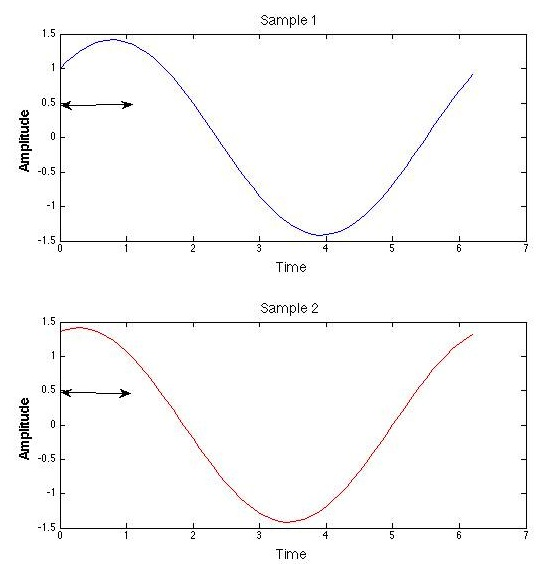
\includegraphics[scale=0.4]{Example1.jpg}
  \caption{Two signals separated by translation}
 \end{figure}
The signal denoted by the `red' color is a `slower' version of the signal denoted by the `blue' color . In the above example, if we are comparing the similarity  between the  time slices spanned by the arrows, an ideal kernel must be invariant to  the time offsets of the signals and thus should consider all possible pairings between the vectors in the subsequences. Intuitively speaking, the kernel must behave like a DTW algorithm..\\
\begin{figure}[h!]
  \centering
   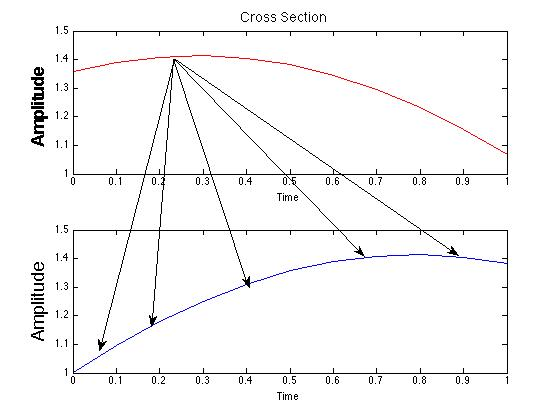
\includegraphics[scale=0.6]{Cross-section.jpg}
  \caption{Two identical subsequences varying in time }
  \end{figure}
 For time slices of width $n$, the kernel  metric  can be expanded and   expressed as :
\begin{eqnarray*}
k(x,z) &= &<\sum_{i=1}^{n}x_i, \sum_{j=1}^{n}z_i>\\
&  =& <(x_1+x_2+x_3+..),(z_1+z_2+z_3+..)>\\
&= & <x_1,z_1>+<x_1,z_2>+<x_1,z_2>...+<x_2,z_1>+<x_2,z_2> +<x_2,z_3>+......\\ 
\end{eqnarray*}
From above expression, we can see  that the proposed kernel corresponds to a sum of all possible dot products of pairs belonging to the set
$\{(x_iz_i) | x_i\in \mbox{seq1}, z_i \in \mbox{seq2}\}$. Similar to the polynomial kernel, the proposed kernel  allows us to match all possible pairs of vectors belonging to the two sub-sequences  given by the matrices.
It is easy to check that this proposed kernel is in fact a valid kernel:
\begin{itemize} \itemsep-2pt
\item K(x,z)= K(z,x) $\Rightarrow $the function is symmetric.
\item The kernel satisfies Mercer's theorem : K(x,z) =$\phi(x)^T\phi(x)$
where  the feature mapping corresponds to  a finite summation of vectors $\phi(y) = \sum_{i=1}^{n}y_i$. 
\end{itemize}

Augmenting the kernel to the DTW algorithm allows DTW to work on high-dimensional time sequences with using a window constraint. However the accuracy and computational cost of the DTW is now dependent on the size of the time slices used to segment the original sequences:
\begin{itemize} \itemsep-2pt
\item The accuracy of DTW increases as the width of the windows decrease. Using subsequence allows the similarity measure to be dominated by the dot products of points whose local and global features are most alike. However using smaller windows achieve lesser dimensionality reduction. Thus the time and computational complexity suffers.
\end{itemize}
To use this kernel as an  appropriate cost function in the DTW algorithm, we need a functional mapping that:
\begin{enumerate} \itemsep-2pt
\item  constraints the codomain to be in the range from 0 to $\infty$.
\item    ensures larger values given by the function signify great degree of dissimilarity and smaller values  signify a high degree of similitude.
\end{enumerate}
An ideal cost function that make use of dot product sis the \emph{arc-cosine}. Hence I embedded the kernel function in the cosine distance: 
\[ \theta = \frac{ <X,Z>}{|X||Z|} \]
where $X = \sum_{i=1}^{n}x_i$ and $Z =\sum_{j=1}^{n}z_i$

A formal outline of the algorithm is as follows:

 \begin{algorithm}
\begin{algorithmic}[1]
\Procedure{Value-based}{$seq1,seq2$}\Comment{two sequences of feature vectors}
\State  seq\_1$\leftarrow$segment(seq1,n)\Comment{ Segment the sequences using a window of size n}
 \State seq\_2$\leftarrow$segment(seq2,n)
 \For{i=1: to length(seq\_1) } \Comment{Initialise the DTW cost matrix}
 \State DTW(i,0) = $\infty$
 \EndFor
 
 \For{i=1 to length(seq\_2)}
 \State DTW(0,i) = $\infty$
 \EndFor
  \For{i=2 to length(seq\_1)}  
 \For{j=max(2, i-w) to min(length(seq\_2), i+w)} 
 
  \State DTW(i,j) = $\theta = \frac{ <X,Z>}{|X||Z|} $+ min\{ DTW(i-1,j)+DTW(i,j-1)+DTW(i-1,j-1)\}
 \EndFor \Comment { $X = \sum_{i=1}^{n}x_i$ and $Z =\sum_{j=1}^{n}z_i$}

 
 \EndFor
\State \textbf{return}  result = $\frac{\mbox{DTW(n,m)}}{nm}$ \Comment{n=length(seq1), m=length(seq2)}

\EndProcedure
\end{algorithmic}
\caption{Adapted DTW}
\end{algorithm}
 

\newpage

\section{Experimental results}
The changes that I have introduced,  in the previous section  to the `Dynamic Time Warping' algorithm is aimed to improve the algorithm's performance in handling high dimensional time series data. In this section, I investigate the investigate the performance of my proposed algorithm by running it  on the test data set that I have constructed from TIDIGITS test corpus and the time complexities and accuracies  against the methodologies that I have investigated so far:
 
\begin{itemize}
\item Approach 1
\begin{itemize}
\item Apply feature selection process to remove segments of silence and down sample the remaining segment to improve the quality.
\item  Apply value-based DTW(which we denote as baseline) using the most constrained window size  and a euclidean metric.
\end{itemize}

\item Approach 2
\begin{itemize}
 \item Apply no feature selection process
 \item Perform feature extraction by extracting MFCC features
 \item Apply DTW using the most constrained window size and a euclidean metric.
 \end{itemize}
 
 \item  Approach 3
 \begin{itemize}
 \item Apply feature selection process that only removes  segments of  silence 
 \item Extract MFCC features
 \item Apply DTW augmented with the euclidean metric.
 \end{itemize}

 
\item Approach 4
\begin{itemize}
\item Apply feature selection process to remove segment of utterance and down sample the remaining segment to improve the quality.
\item Apply  the feature extraction process discussed in [3.2.1] to extract local and global features.
 \item Apply DTW using the most constrained window size  and a euclidean metric.
 \end{itemize}


 
 
 \end{itemize}


\begin{figure}[h!]
  \centering
   
     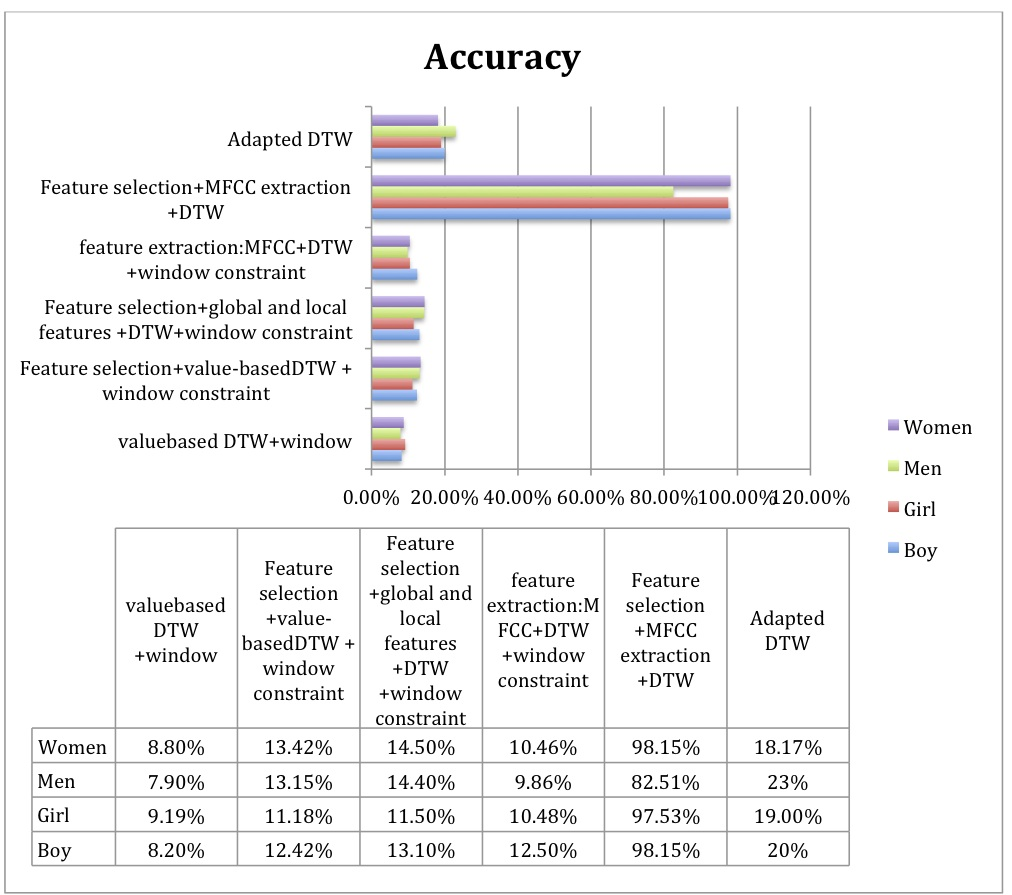
\includegraphics[scale=0.8]{AdaptedDTW-accuracy.jpg}
  \caption{Accuracy}
  
\end{figure}

\begin{figure}[H]
  \centering
   
   
     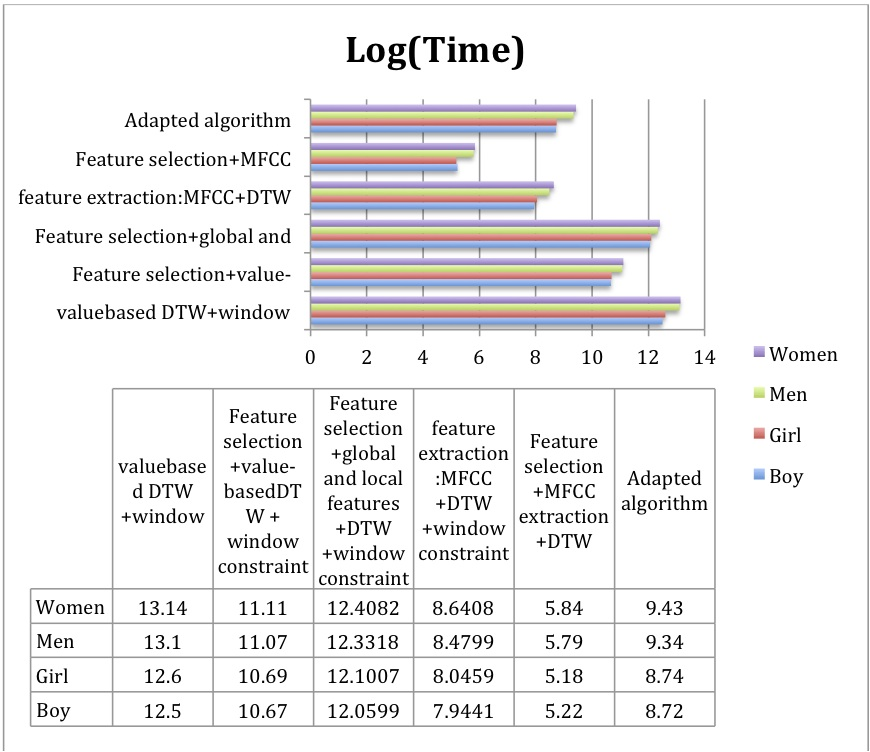
\includegraphics[scale=0.8]{AdaptedDTW-time.jpg}
  \caption{Time complexity}
  \end{figure}

There are quite number of interesting observations that can made from the graphs and the tables given by figures [4.3,4.4]. 

\begin{itemize}
\item The proposed algorithm achieves better accuracy for test samples belonging to all categories than any of algorithms that employ the rigid  window constraint of  $w = max(\lceil{0.1*max(n.m)}\rceil, abs(n-m))$. The most interesting result is that the new algorithm incurs a lower computational cost than any of these DTW algorithms. 
\item From examining the improvements in accuracy across all categories, it can be concluded that for the TIGITS dataset,  the new algorithm is invariant to variations introduced  in the acoustic signals  by different speakers . 
\item The  methodology behind my proposed approach and that of  approach 4  includes the same pre-processing stage. Th input to the DTW algorithm is constructed by using  the domain dependent feature selection process mentioned in section followed by a domain independent feature extraction mapping (i.e the local and global features defined in section).  Both approaches  differ however, in their use of a cost function and a window constraint. The proposed approach doesn't subject DTW  to any window constraints and utilised the kernel function that I constructed in the cost metric. Approach 4 on the other hand, employs the euclidean metric an subjects DTW to the window constraint of  of w = max($\lceil{0.1*max(n.m)}\rceil$, abs(n-m))
The proposed DTW segments sequences into frames and employ a cost function on  the frames. This reduces the dimensionality of the time series sequences and allows the algorithm to achieve a  time and computational cost than is lower than  the cost incurred by any of the investigated adaptations of the DTW algorithm that  employs window constraints. 
\end{itemize}

  To confirm that the performance of the new algorithm  is not tailored for this particular time-series data set, I have applied the tested the algorithm on the two largest  time series data sets in UCR database. 
  
    Unlike the speech utterances, the time series sequences within each data set  share the same length.
  
  \subsection{Experimental setup}
  
 The focus now is  to check how well/ bad is the performance of the new DTW algorithm  against  DTW algorithms using window constraints when applied to datasets that belong to other application domains . The domain -dependent pre-processing policies are dropped for this set of experiments as these procedures were specifically designed for speech data. Thus in this section, I compare my proposed approach against:
 \begin{itemize}
 \item Approach 1
 \item Approach 4 
 \end{itemize}
  As a I mentioned, the domain-dependent feature selection process  of silence removal and subsampling is dropped from all approaches. However, the feature extraction process  that involves extracting  local and global features is kept since this procedure is domain independent.
  
One of the factors that I have also investigated in these experiments is  the size of the time slices used in the algorithm that I proposed. For the TIDIGITS data set, I have used window slices of 50 ms. Reducing the size of the windows should principally increase both accuracy and time-complexity .
The core kernel used by the new algorithm is based on the function: 
\[ k(x,z) = <\sum_{i=1}^{n}x_i, \sum_{j=1}^{n}z_j>\]
k(x,z) represents the sum of all possible dot-products . Having a smaller window allows the sum to be dominated by dot products of vectors that are most similar. However smaller window  frames results in  longer time series sequence of frames. This in turn increases the time and computational complexity incurred by the DTW algorithm.
  
Figure [4.5] and figure[4.6] shows the  accuracies and log(time) of the  algorithms  for the two datasets:

  \begin{figure}[H]
  \centering
   
     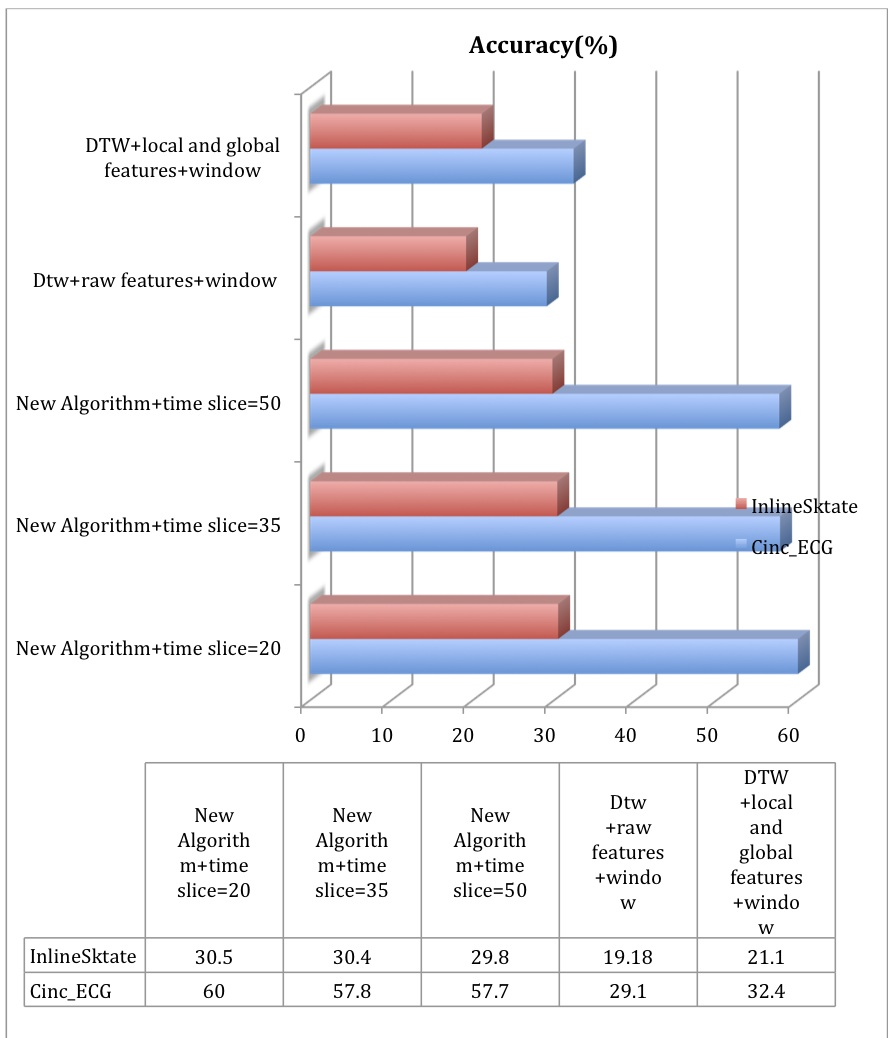
\includegraphics[scale=0.8]{accuracy_cinc_inline.jpg}
  \caption{Accuracy}
  \end{figure}
   
   Observation:
   \begin{itemize}
   \item The  new algorithm indeed achieves better accuracy than any versions of the window  constrained DTW algorithm employing domain-independent feature extraction
   \item Comparatively, the performance of the new algorithm does improve if smaller window slices are employed to partition the time series sequence of vectors. 
   \end{itemize}
   
   
\begin{figure}[H]
  \centering
   
     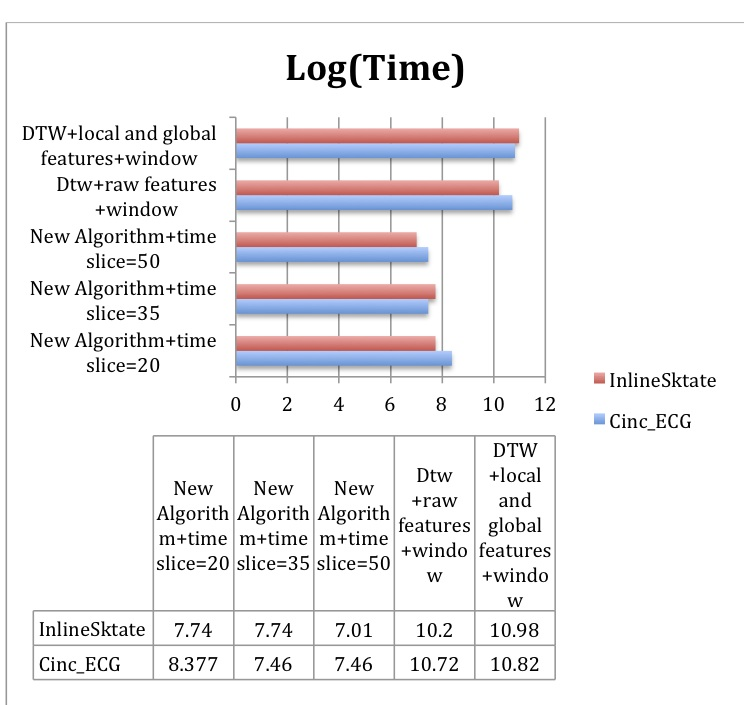
\includegraphics[scale=0.8]{time_cinc_inline.jpg}
  \caption{Time complexity}
  \end{figure}
Observation:
   \begin{itemize}
   \item The  new algorithm incurs less time and computational cost  than any versions of the window  constrained DTW algorithm employing domain-independent feature extraction
   \item Comparatively, the time complexity of the new algorithm increases when smaller window slices are used to partition the sequence
   \end{itemize}   



%% ... etc ...

%%%%%%%%
%% Any appendices should go here. The appendix files should look just like the
%% chapter files.
%\appendix

\include{appendix1}

%% ... etc...

%% Choose your favourite bibliography style here.
\bibliographystyle{apalike}

%% If you want the bibliography single-spaced (which is allowed), uncomment
%% the next line.
% \singlespace

%% Specify the bibliography file. Default is thesis.bib.
\bibliography{thesis}
% 100 is a random guess of the total number of 
%references
\begin{thebibliography}{100} 

\bibitem {} Das, G., Lin, K., Mannila, H., Renganathan, G. & Smyth, P. 
(1998). ``\emph{Rule discovery from time series}''. In proceedings of 
the 4th Int'l Conference on Knowledge Discovery and Data 
Mining. New York, NY, Aug 27-31. pp 16-22.
\bibitem{} Ying Xie, Bryan Witgen ``\emph{Adaptive Feature Based Dynamic Time Warping}'',International Journal of Computer Science And Network Security, January 2010.
\bibitem{} Alex S .Park James R.Glass \emph{Unsupervised Pattern Discovery in Speech},
IEEE Transactions On Audio Speech  And Language Processing, VOL 16, January 2008.
\bibitem{} Mathias De Wachter, Mike Matton, Kris Demuynck, Patrick Wambacq ``\emph{Template Based Continuous Speech Recognition}"  IEEE Transactions On Audio And Speech Processing ,2007.
\bibitem{}  Yaodang Zhang and James R.Glass ``\emph{Towards Multi-Speaker Unsupervised Speech Pattern Discovery}" in Proc 2009.
\bibitem{}  Yaodang Zhang and James R.Glass "\emph{ Unsupervised spoken keyword spotting via segmental DTW on Gaussian Posterior-grams}" in Proc 2009.
\bibitem{} Mathias De Wachter, Mike Matton, Kris Demuynck, Patrick Wambacq "\emph{A Locally Weighted Distance Measure For Example Based Speech Recognition}" ICASSP 2004.
\bibitem{}Michael A .Carlin, Samuel Thomas, Aren Jansen, Hyek Hermansky  ``\emph{Rapid Evaluation of Spoken Term Discovery} ",  INTERSPEECH 2011: 821-824.
\bibitem{} Hui Zhang, Tu Bao ho, Yang Zhang, Mao-Song-Lin ``\emph{Unsupervised Feature Extraction for Time Series Clustering Using Orthogonal Wavelet Transform}"   Informatica 30(2006) 305-319.
\bibitem{} S.Mallet ``\emph{ A Wavelet  Tour of Signal Processing}" Academic Press ,San Diego ,second edition,1999.
\bibitem{} ] A. Brazma, I. Jonassen, I. Eidhammer, and D. Gilbert,  ``\emph{Approaches to
the automatic discovery of patterns in biosequences} "  J. Comput. Biol.,vol. 5, no. 2, pp. 279�305, 1998.
\bibitem{}F Korn, H. Jagadish  and C.Faloutos. ``\emph{Efficiently supporting ad hoc queries in large datasets of time sequences}". In Proceedings of the ATM of the ACM SIGMOID International Conference of  Management Of Dat, pages 289-300.
\bibitem{}Chun-Lin, Liu ``\emph{ A Tutorial of the Wavelet Transform}" February 23, 2010.
\bibitem{} Josif Grabocka, Erind Bedalli and Lars Schmidt-Thiem ``\emph{ Efficient  Classification of Long Time-Series}", Information Systems and Machine Learning Lab.ICT Innovations 2012, pages 47-57.
\bibitem{}Jessica Lin Eamonn Keogh Stefano Lonardi Pranav Patel ``\emph{Finding Motifs in Time Series}", CiteSeer 2002.
\bibitem {} Lee A.Barford, R. Shane Fazzio, DavidR. Smith Instruments and Photonics Laboratory ``\emph{An Introduction to Wavelets}"  September, 1992.
\bibitem{} Fayyad, U., Reina, C. &. Bradley. P (1998). ``\emph{Initialisation of  iterative refinement clustering algorithms}''. In Proceedings of the 4th International Conference on Knowledge Discovery and Data Mining. New York, NY, Aug 27-31. pp 194-198
\bibitem {} Sakoe, H. & chiba, S. (1978). ``\emph{ Dynamic programming algorithm optimization fro spoken word }" Trans. Acoustics, Speech, and Signal Proc., Vol. ASSP-26. pp. 
43-49. 
\bibitem{}Itakura, F. (1975). ``\emph{Minimum prediction residual principle applied to speech recognition}". IEE Speech, and Signal Proc., Vol. ASSP-23, pp. 52-72. 
\end{thebibliography} 
\bibitem{}Fu, A.W., Keogh, E., Lau, L.Y.H., & Ratanamahatana, C.A. (2005). ``\emph{Scaling and Time Warping in Time Series Querying}". VLDB �05, pp. 649-660. 
\bibitem{}Xiaopeng  Xi, Eamonn Keogh, Christian Shelton, Li Wei  ``\emph{Fast Time Series Classification Using Numerosity Reduction}" ICML '06 Proceedings of the 23rd international conference on Machine learning Pages 1033-1040 
\bibitem{} D. Kim and B. Yum, ``\emph{Collaborative Filtering Based on Iterative Principal Component Analysis}�, Expert Systems with Applications 28 (2005), 823�830.
%% ... that's all, folks!
\end{document}
